\subsection{Three-Dimensional Tradeoff: Tag Length, Witness Cost, Distortion}

Recall from Section 2 that observer strategies are characterized by three dimensions:
\begin{itemize}
\item \textbf{Tag length} $L$: bits required to encode a class identifier ($L \geq \log_2 k$ for $k$ classes under full class tagging)
\item \textbf{Witness cost} $W$: minimum number of primitive queries for class identification
\item \textbf{Distortion} $D$: probability of misclassification, $D = \Pr[\hat{C} \neq C]$.
\end{itemize}

We compare two observer classes:

\begin{definition}[Attribute-only observer]
An observer that queries only attribute membership ($q_I \in \Phi_{\mathcal{I}}$), with no access to explicit class tags.
\end{definition}

\begin{definition}[Nominal-tag observer]
An observer that may read a single class identifier (nominal tag) per value, in addition to attribute queries.
\end{definition}

\begin{theorem}[Pareto Optimality of Nominal-Tag Observers]\label{thm:lwd-optimal}
Let $A_\pi$ be the collision multiplicity (Definition~\ref{def:collision-multiplicity}). Then:
\begin{enumerate}
\item Any $D=0$ scheme must satisfy $L \ge \log_2 A_\pi$ (Theorem~\ref{thm:converse}).
\item In maximal-barrier domains ($A_\pi = k$), nominal-tag observers achieve the unique Pareto-optimal $D=0$ point:
\begin{itemize}
\item \textbf{Tag length}: $L = \lceil \log_2 k \rceil$ bits for $k$ classes
\item \textbf{Witness cost}: $W = O(1)$ queries (one tag read)
\item \textbf{Distortion}: $D = 0$ (zero misclassification probability)
\end{itemize}
\item In general (non-maximal) domains, nominal tagging remains Pareto-optimal at $D=0$ but need not be unique: partial tags can coexist on the frontier.
\end{enumerate}

In information-barrier domains, attribute-only observers (the $L=0$ face) satisfy:
\begin{itemize}
\item \textbf{Tag length}: $L = 0$ bits (no explicit tag)
\item \textbf{Witness cost}: $W = \Omega(d)$ queries (must query at least one minimal distinguishing set of size $d$, see Definition~\ref{def:distinguishing-dimension})
\item \textbf{Distortion}: $D > 0$ (probability of misclassification is strictly positive due to collisions)
\end{itemize}
\end{theorem}

\begin{proof}
Converse item (1) is Theorem~\ref{thm:converse}. For item (2), maximal barrier means all classes are observationally colliding, so any $D=0$ scheme must carry full class identity in tag bits (Corollary~\ref{cor:max-barrier-converse}), while nominal tags realize this lower bound with one tag read. Pareto uniqueness follows because any competing $D=0$ point cannot reduce $L$ below $\log_2 k$ nor reduce $W$ below constant-time tag access under the admissibility rules of Section~\ref{sec:framework}.

The converse proof path is machine-checked in Lean: \texttt{proofs/lwd\_converse.lean} formalizes (i) constant transcript on a collision block implies tag injectivity under zero-error decoding, and (ii) counting then yields $2^L \ge A_\pi$. The maximal-barrier corollary is formalized in the same module. Runtime cost instantiations (e.g., unbounded gap examples) remain in \texttt{proofs/python\_instantiation.lean}.
\end{proof}

\begin{remark}[General $D=0$ Frontier]
When $1 < A_\pi < k$, the $D=0$ frontier can include mixed designs: a partial tag identifies collision blocks and queries resolve within blocks. This does not contradict nominal optimality; it only removes global uniqueness outside maximal-barrier domains.
\begin{enumerate}
\item Maximal barrier ($A_\pi=k$): unique $D=0$ nominal point.
\item Intermediate barrier ($1<A_\pi<k$): multiple $D=0$ Pareto points may exist.
\item No barrier ($A_\pi=1$): $L=0$ zero-error identification is feasible.
\end{enumerate}
\end{remark}

\subsection{Pareto Frontier}

The three-dimensional frontier shows:
\begin{itemize}
\item In maximal-barrier domains, the unique $D=0$ Pareto point is nominal tagging at $L=\lceil \log_2 k\rceil$.
\item In general domains, attribute-only observers trade tag length for distortion on the $L=0$ face when collisions are present.
\end{itemize}

Figure~\ref{fig:lwd-tradeoff} visualizes the $(L, W, D)$ tradeoff space. The key observation is the ambiguity converse: the minimum zero-error tag rate is $\log_2 A_\pi$, with the maximal-barrier special case $\log_2 k$.

\begin{figure}[t]
\centering
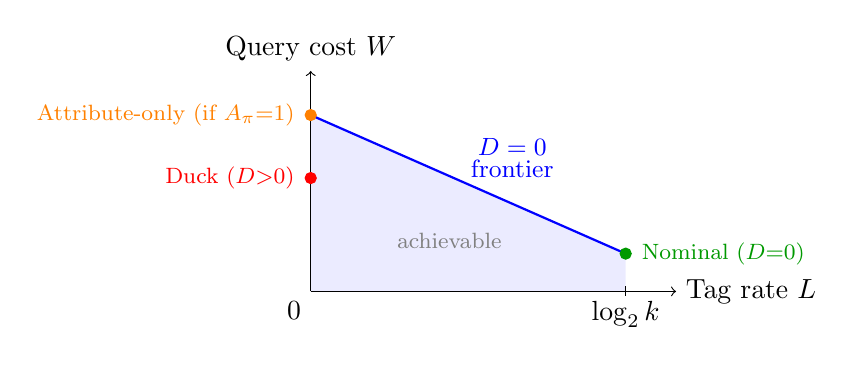
\begin{tikzpicture}[scale=0.8]
  % Shaded D=0 achievable region (draw FIRST)
  \fill[blue!8] (0,0) -- (5,0) -- (5,0.6) -- (0,2.8) -- cycle;

  % D=0 Pareto frontier
  \draw[thick, blue] (0,2.8) -- (5,0.6);

  % Axes (draw after shading)
  \draw[->] (0,0) -- (5.8,0) node[right] {Tag rate $L$};
  \draw[->] (0,0) -- (0,3.5) node[above] {Query cost $W$};

  % Axis labels
  \node[below left] at (0,0) {$0$};
  \node[below] at (5,0) {$\log_2 k$};
  \draw (5,0.08) -- (5,-0.08);

  % Region labels
  \node[blue] at (3.2,2.3) {\small $D = 0$};
  \node[blue] at (3.2,1.95) {\small frontier};
  \node[gray] at (2.2,0.8) {\footnotesize achievable};

  % Points on the D=0 frontier
  \filldraw[orange] (0,2.8) circle (2.5pt);
  \node[orange, left] at (-0.1,2.8) {\footnotesize Attribute-only (if $A_\pi{=}1$)};

  \filldraw[green!60!black] (5,0.6) circle (2.5pt);
  \node[green!60!black, right] at (5.1,0.6) {\footnotesize Nominal ($D{=}0$)};

  % Duck typing: below frontier, accepts D>0
  \filldraw[red] (0,1.8) circle (2.5pt);
  \node[red, left] at (-0.1,1.8) {\footnotesize Duck ($D{>}0$)};

\end{tikzpicture}
\caption{Schematic illustration of the $(L, W, D)$ tradeoff. For a concrete example with $k = 1000$ classes, distinguishing dimension $d = 10$, and maximal barrier ($A_\pi = k$), the nominal-tag strategy achieves $L = 10$ bits, $W = O(1)$, $D = 0$, while the attribute-only strategy requires $W = 10$ queries and incurs $D > 0$ due to collisions.}
\label{fig:lwd-tradeoff}
\end{figure}

The Lean 4 formalization (Appendix~\ref{sec:lean}) machine-checks the full ambiguity-based converse chain and maximal-barrier lower bound that anchor this tradeoff analysis.

\begin{remark}[Programming language instantiations]
In programming language terms: \emph{nominal typing} corresponds to nominal-tag observers (e.g., CPython's \texttt{isinstance}, Java's \texttt{.getClass()}). \emph{Duck typing} corresponds to attribute-only observers (e.g., Python's \texttt{hasattr}). \emph{Structural typing} is an intermediate case with $D = 0$ but $W = O(n)$.
\end{remark}

\begin{remark}[Structural-check cost parameter]
When structural typing checks traverse $s$ members/fields (rather than ranging over the full attribute universe), the natural bound is $W = O(s)$ with $s \le n$.
\end{remark}
